\documentclass[]{lapesd-thesis}

% Outros \usepackage{}

%%%%%%%%%%%%%%%%%%%%%%%%%%%%%%%%%%%%%%%%%%%%%%%%%%%%%%%%%%%%%%%%%%%%
%%% Configurações da classe (dados do trabalho)                  %%%
%%%%%%%%%%%%%%%%%%%%%%%%%%%%%%%%%%%%%%%%%%%%%%%%%%%%%%%%%%%%%%%%%%%%

% Informações para capa e folha de rosto/certificacao
\titulo{Comparação das tecnologias de comunicação entre clusters 
no processador MPPA-256 atráves do CAP Benchmarks}
\autor{David Grunheidt Vilela Ordine}
\data{\today}
\tcc
\departamento{Departamento de Informática e Estatística}
\curso{Ciências da Computação}
\titulode{Bacharel em Ciência da Computação}
\orientador{Prof. Márcio Bastos Castro, Dr.}
\coorientador{Pedro Henrique Penna, Dr.}
\afiliacaocoorientador{Université Grenoble Alpes}

%%% Atenção! No caso de TCC, além de usar \tcc, outros comandos devem ser 
%%% fornecidos:
% \tcc
% \departamento{Departamento de Informática e Estatística}
% \curso{Ciência da Computação}
% \titulode{Bacharel em Ciência da Computação}
% %% Para TCCs, orientadores e coorientadores podem ser externos, logo a
% %% BU exige que sua afiliação seja explicitada. Por padrão, assume-se
% %% UFSC. Você pode alterar a afiliação com os comandos abaixo:
% \afiliacaoorientador{Universidade Federal de Santa Catarina}
% \afiliacaocoorientador{Universidade Federal da Terra de Ninguém}

% Membros da banca e coordenador
% As regras da BU agora exigem que Dr. apareça depois do nome
% Dica: para gerar Profᵃ. use Prof\textsuperscript{a}.
% Dica 2: para feminino use \orientadora e \coorientadora
\membrobanca{Prof. Prof1, Dr.}{Universidade Federal de Santa Catarina}
\membrobanca{Prof. Prof2, Dr.}{Universidade Federal de Santa Catarina}
\membrobanca{Prof. Prof3, Dr.}{Universidade Federal de Santa Catarina}
\coordenador{Prof. José Francisco Danilo de Guadalupe Correa Fletes, Me.}


% Ativa indíce remissivo. Precisa estar aqui, não funciona no .cls nem no
% \BeforeBeginDocument{}
\makeindex
% Carrega definições dos acrônimos e do glossário. Isso precisa ser feito antes
% do \begin{document}

%%%%%%%%%%%%%%%%%%%%%%%%%%%%%%%%%%%%%%%%%%%%%%%%%%%%%%%%%%%%%%%%%%%%
%%% Lista de acronimos                                           %%%
%%%%%%%%%%%%%%%%%%%%%%%%%%%%%%%%%%%%%%%%%%%%%%%%%%%%%%%%%%%%%%%%%%%%
%%% Importante:                                      
%%% - A lista PRECISA SER MANTIDA ORDENADA
%%%%%%%%%%%%%%%%%%%%%%%%%%%%%%%%%%%%%%%%%%%%%%%%%%%%%%%%%%%%%%%%%%%%

\tnewacronym{APE}{Application Programming Interface}
            % \APE e \APEs nunca espandem, mas ele aparece na lista de siglas
\xnewacronym{DHT}{Distributed Hash Table}
            % Se \DHTs for o primeiro uso, Tabe ganha um s no final
\xnewacronym[][longplural={Square Matrices}]{SQ}{Square Matrix}
               % trata o plural usado em \SQs
               % note que como queremos passar o 2o arg opcional, devemos 
               % passar o primeiro (podemos deixar em branco)
\xnewacronym[WTC]{W3C}{World Wide Web Consortium}
            % gera comando \WTC que expande para "World ... (W3C)"

\xnewacronym{HPC}{High-Performance Computing}

\xnewacronym{API}{Application Programming Interface}

\xnewacronym{IPC}{MPPA Interprocess Communication API}

\xnewacronym{ASYNC}{MPPA Asynchronous Communication API}

\xnewacronym{Flops}{Floating-point Operations per Second}

\xnewacronym{RAM}{Random-Access Memory}

\xnewacronym{CPU}{Central Processing Unit}

\xnewacronym{UMA}{Uniform Memory Access}

\xnewacronym{NUMA}{Nonuniform  Memory  Access}

\xnewacronym{CMP}{Chip MultiProcessadores}

\xnewacronym{GPU}{Unidade de Processamento Gráfico}

\xnewacronym{SIMD}{Single  Instruction  Multiple Data}

\xnewacronym{SO}{Sistema Operacional}

\xnewacronym[][longplural={Clusters de Computação}]{CC}{Cluster de Computação}

\xnewacronym[IO]{E/S}{Entrada e Saída}

\xnewacronym{OpenMP}{Open Multi-Processing}

\xnewacronym{MPI}{Message Passing Interface}

\xnewacronym{SPMD}{Single Program, Multiple Data}

\xnewacronym{NoC}{Network-on-Chip}

%%% Local Variables:
%%% mode: latex
%%% TeX-master: "main"
%%% End:


%%%%%%%%%%%%%%%%%%%%%%%%%%%%%%%%%%%%%%%%%%%%%%%%%%%%%%%%%%%%%%%%%%%%
%%% Glossario                                                    %%%
%%%%%%%%%%%%%%%%%%%%%%%%%%%%%%%%%%%%%%%%%%%%%%%%%%%%%%%%%%%%%%%%%%%%
%%% Importante:                                      
%%% - A lista PRECISA SER MANTIDA ORDENADA
%%%%%%%%%%%%%%%%%%%%%%%%%%%%%%%%%%%%%%%%%%%%%%%%%%%%%%%%%%%%%%%%%%%%

\xnewglossaryentry{polling}{%
  name={polling},%
  description={A type of event delivery technique consisting of the consumer repeatedly asking the provider for the most recent events}%
}
\xnewglossaryentry{proxy}{%
  name={proxy},%
  plural={proxies},%
  description={A proxy shapiro1986 encapsulates remote servers and provides a single view to their services. The proxy can then intercept communication and provide additional functionality, such as message translation and performance enhancement. The client must take the initiative of selecting and using a proxy [p.~46,97]fielding2000.}%
}

%%% Local Variables:
%%% mode: latex
%%% TeX-master: "main"
%%% End:


\begin{document}

%%%%%%%%%%%%%%%%%%%%%%%%%%%%%%%%%%%%%%%%%%%%%%%%%%%%%%%%%%%%%%%%%%%%
%%% Conteúdo                                                     %%%
%%%%%%%%%%%%%%%%%%%%%%%%%%%%%%%%%%%%%%%%%%%%%%%%%%%%%%%%%%%%%%%%%%%%

\pretextual%
\newcommand{\mppa}{MPPA-256\xspace}
\newcommand{\capb}{CAP Bench\xspace}
\newcommand{\epiphany}{Adapteva Epiphany\xspace}
\newcommand{\manycore}{\textit{manycore}\xspace}
\newcommand{\manycores}{\textit{manycores}\xspace}
\newcommand{\bench}{\textit{benchmark}\xspace}

% Assume-se que \pretextual já foi feito

\imprimircapa%
\imprimirfolhaderosto*
% Atenção! esse \protect é importante
\protect\incluirfichacatalografica{ficha.pdf}
\imprimirfolhadecertificacao


\begin{dedicatoria}
  Este trabalho é dedicado a minha família, que sempre me apoiou e esteve do meu lado, e também aos meus amigos, os quais me ajudaram a passar por todo o processo de escrita e implementação de uma maneira mais feliz.
\end{dedicatoria}


\begin{agradecimentos}
  Agradeço a todos os meus colegas de trabalho e de curso, os quais contribuíram significativamente para a conclusão deste trabalho, através da troca de experiência e conhecimentos técnicos. Em especial, agradeço ao meu orientador, Márcio Bastos Castro, e meu co-orientador, Pedro Henrique Penna, por despertarem em mim interesse na área da computação paralela e me ajudarem no processo de aprendizado e desenvolvimento deste trabalho.
\end{agradecimentos}


\begin{epigrafe}
  For a number of years I have been familiar with the observation that the quality of programmers is a decreasing function of the density of go to statements in the programs they produce \\
  \cite{dijkstra1968}
\end{epigrafe}


\begin{resumo}[Resumo]
  O principal método para o ganho em desempenho, no processo de evolução dos processadores \textit{single-core}, foi o aumento da frequência de \textit{clock} do processador, o qual, com a crescente desproporção entre o gasto energético e o aumento de performance, deixou de ser viável. Diz-se então que esta desproporção foi a barreira de evolução para esta classe de processadores. Soluções que utilizam processadores \textit{multi-core}, por exemplo, supercomputadores, também enfrentam uma barreira similar, nos dias de hoje, ao agrupar diversos destes processadores em \textit{clusters}, ou agrupar diversos núcleos em um mesmo \textit{chip}. Processadores \manycore de baixo consumo energético, como o \mppa e o \epiphany, surgiram como uma possível solução para este problema. Entretanto, devido a questões arquiteturais, como uma memória distribuída e limitada no \textit{chip}, a implementação de uma aplicação que beneficia-se totalmente do \textit{hardware} de um processador desta classe mostra-se desafiadora. Porém, quando bem feita, sobressai alguns processadores \textit{multi-core} do estado da arte, através do menor consumo energético. Neste projeto foram propostas para o \capb, um \bench desenvolvido para avaliar o desempenho e o consumo de energia do \mppa, otimizações nas aplicações da versão atual e a criação de uma versão das aplicações que utiliza uma nova tecnologia de comunicação assíncrona entre \textit{clusters}, com objetivo de analisar as duas tecnologias de cada versão. Os resultados até o momento mostram que as aplicações que utilizam a nova biblioteca apresentam melhor desempenho sobre as aplicações da versão antiga. Isso se deve principalmente pela característica assíncrona desta biblioteca.



  % Atenção! a BU exige separação através de ponto (.). Ela recomanda de 3 a 5 keywords
  \vspace{\baselineskip} 
  \textbf{Palavras-chave:} Benchmark. Manycore. Desempenho. Green-Computing.
\end{resumo}


\begin{resumo}[Resumo Estendido]
%%%%%%%%%%%%%%%%%%%%%%%%%%%%%%%%%%%%%%%%%%%%%%%%%%%%%%%%%%%%%%%%%%%%%%
% Atenção: normas e templates contraditórios!!!                    %%%
%%%%%%%%%%%%%%%%%%%%%%%%%%%%%%%%%%%%%%%%%%%%%%%%%%%%%%%%%%%%%%%%%%%%%%
% - Modelo da BU: https://repositorio.ufsc.br/handle/123456789/197458
% - A BU exige no **mínimo** 2 páginas e no **máximo** 5
% - Regimento do PPGCC, Art 40 Entende-se  por  resumo  estendido  um  documento  que  contenha  as  informações  mais  relevantes  de  cada  capítulo  da  tese  ou  da  dissertação.
% O mais seguro é ignorar o regimento e seguir a BU.
    % Atenção! A BU diz que o resumo **deve** conter as seções abaixo!
\section*{Introdução} % Deve ser  subsection*, devido a formatação usada no modelo

Similar ao que aconteceu com os sistemas que utilizavam processadores \textit{single core}, os supercomputadores da atualidade estão se deparando com uma barreira que impede o avanço em direção ao \textit{Exascale}. A principal causa deste impedimento tem relação com as características intrínsecas da arquitetura de processadores \textit{multicore} que compõem muitos destes supercomputadores. Assim como processadores \textit{singlecore} não puderam mais aumentar a frequência de clock de um núcleo após um certo limite, só é possível diminuir o tamanho dos transistores que formam um núcleo de processamento até um certo ponto, e da mesma maneira, só é possível alocar uma certa quantidade de núcleos em um \textit{chip}, antes que o gerenciamento desses núcleos fique algo inviável de ser implementado ou o tamanho do \textit{chip} fique muito grande. Além disso, ao longo do tempo a relação entre dissipação de calor e ganho em performance mostrou-se não escalável para esta arquitetura. Assim, a comunidade científica de \HPC começou a pesquisar e desenvolver novas arquiteturas que apresentassem melhor escalabilidade entre as variáveis citadas acima, surgindo então a classe de processadores \textit{manycore} de baixo consumo energético, por exemplo, o MPPA-256, que será estudado neste trabalho.

\section*{Fundamentação Teórica} 
Atualmente, arquiteturas com múltiplos processadores são algo comum em diversos sistemas, porém, nem todos sabem como caracterizar estes sistemas de acordo com a disposição dos elementos que os compõem. Dentre essas arquiteturas, temos os sistemas multiprocessadores e os multicomputadores, sendo a principal diferença entre eles o compartilhamento ou não de memória por parte dos núcleos de processamento. Enquanto os sistemas de multiprocessadores conectam esses núcleos a uma memória através de um barramento, os multicomputadores conectam as unidades de processamento através de uma rede, onde cada unidade tem sua memória privada, e a comunicação entre as unidades é feita via troca de mensagens através de alguma API. Além disso, os multiprocessadores podem ser divididos em duas categorias, os UMA e NUMA, onde o que os difere é o tempo de acesso a uma palavra na memória ser o mesmo ou não, para qualquer palavra. Vale citar que o MPPA-256, processador usado neste trabalho, se enquadra na classe dos multiprocessadores. Para estes sistemas existem diversas bibliotecas e padrões voltados a programação paralela, sendo os mais comuns o MPI, padrão o qual bibliotecas de troca de mensagem entre processos se baseiam, e a OpenMP, API muito usada quando o assunto é \textit{multithreading}. Ambos permitem abstrair qual plataforma o programa paralelo em questão irá executar, o que facilita a implementação deste programa, sendo esse um dos principais motivos pelo qual são amplamente adotados. Já para o MPPA-256, duas bibliotecas são estudadas neste trabalho. A biblioteca IPC, utilizada na primeira versão do \textit{benchmark}, tem um baixo nível de abstração, sendo necessário conhecer vários aspectos da arquitetura do processador para que seja feita uma implementação otimizada e eficiente de alguma aplicação. Já a ASYNC tem um alto nível de abstração e permite a troca de mensagens de modo assíncrono, o que muitas vezes pode ser uma vantagem para determinadas aplicações.

\section*{Trabalhos Correlatos} 
  
\section*{Desenvolvimento} 

\section*{Resultados preliminares} 

\section*{Conclusão}

\vspace{\baselineskip}  % Atenção! manter igual ao resumo
\textbf{Palavras-chave:} Benchmark. Manycore. Desempenho. Green-Computing.
\end{resumo}


\begin{abstract}
Throughout the evolving process of \textit{single-core} processors, the main method to gain performance was to increase the processor \textit{clock} frequency, which led to the growing disproportion between energy consumption and increase in performance, making this method not viable anymore. This disproportion was then the barrier to the evolution of this class of processors. \textit{Multi-core} processors solutions, for example, supercomputers, also face a similar barrier nowadays when grouping this processors into \textit{clusters}, or grouping several \textit{cores} into a single \textit{chip}. Low consumption \manycore processors, for instance, the \mppa and the \epiphany, are arising to solve this problem. However, due to architectural characteristics, such as a limited and distributed memory, implementing applications that fully benefits from the hardware of a processor of this class is not an easy task. Yet, when a good implementation is done, it can outstand state-of-the-art processors, through lower energy consumption. This project proposes to the \capb, a \bench developed to evaluate both \mppa performance and energy consumption, optimizations to its applications and the implementation of a new version, using a new communication technology, based on asynchronous primitives, aiming to analyze the technologies used in each version. The results until now show that the applications that use the new technology have a better performance than the old ones. This is due, mainly, by the asynchronous characteristic of this library.

  \vspace{\baselineskip} 
  \textbf{Keywords:} Benchmark. Manycore. Performance. Green-Computing.
\end{abstract}

\listoffigures*  % O * evita que apareça no sumário
\listoftables*
\listoflistings*  
\listofalgorithms*

\listadesiglas*[5em]

\begin{listadesimbolos}
  $\gets$   & Atribuição \\
  $\exists$   & Quantificação existencial \\
  $\rightarrow$   & Implicação \\
  $\wedge$   & E lógico \\
  $\vee$   & Ou lógico \\
  $\neg$   & Negação lógica \\
  $\mapsto$   & Mapeia para \\
  $\sqsubseteq$   & Subclasse (em ontologias) \\
  $\subseteq$   & Subconjunto: $\forall x\;.\; x \in A \rightarrow x \in B$ \\
  $\langle\ldots\rangle$ & Tupla \\
  $\forall$   & Quantificação universal \\
  mmmmm & Nenhum sentido, apenas estou aqui para demonstrar a largura máxima dessas colunas. Ao abrir o ambiente \texttt{listadesimbolos}, pode-se fornecer um argumento opcional indicando a largura da coluna da esquerda (o default é de 5em): \texttt{\textbackslash{}begin\{listadesimbolos\}[2cm] .... \textbackslash{}end\{listadesimbolos\}} \\
\end{listadesimbolos}

\tableofcontents*%

%%% Local Variables:
%%% mode: latex
%%% TeX-master: "main"
%%% End:

\textual%
% Assume-se que \textual já foi feito

\newcommand{\multicore}{\textit{multicore}\xspace}
\newcommand{\chip}{\textit{chip}\xspace}
\newcommand{\chips}{\textit{chips}\xspace}
\newcommand{\singlecore}{\textit{singlecore}\xspace}
\newcommand{\tradeoff}{\textit{trade-off}\xspace}
\newcommand{\exaescale}{\textit{Exaescale}\xspace}
\newcommand{\greencomputing}{\textit{Green Computing}\xspace}  
\newcommand{\ranking}{\textit{ranking}\xspace}
\newcommand{\bench}{\textit{benchmark}\xspace}
\newcommand{\capb}{CAP Bench\xspace}
\newcommand{\etal}{\textit{et al}.\xspace}
\newcommand{\thread}{\textit{thread}\xspace}
\newcommand{\threads}{\textit{threads}\xspace}
\newcommand{\cache}{\textit{cache}\xspace}
\newcommand{\caches}{\textit{caches}\xspace}
\newcommand{\byte}{\textit{byte}\xspace}
\newcommand{\bytes}{\textit{bytes}\xspace}
\newcommand{\hardware}{\textit{hardware}\xspace}
\newcommand{\transistor}{\textit{transistor}\xspace}
\newcommand{\transistors}{\textit{transistors}\xspace}
\newcommand{\manycore}{\textit{manycore}\xspace}
\newcommand{\hardware}{\textit{hardware}\xspace}

\chapter{Introdução}
\label{ch:introdução}

Na última década, a indústria de semicondutores vem investindo largamente na pesquisa e produção de \chips com múltiplos núcleos de processamento em seu interior, chamados de \multicore. Os avanços nessa indústria, juntamente com a área de arquitetura de computadores, são notados desde a década de 1980 em diante, permitindo um crescimento anual em desempenho de 40\% a 50\% \cite{Larus2008} para uma outra classe de processadores nesse período, os de um único núcleo ou \singlecore. Porém, a necessidade de uma nova classe de processadores mostrou-se eminente ao se atingir um ponto onde o \tradeoff entre gasto energético e aumento em desempenho era desproporcional, havendo muita dissipação de calor para pouco crescimento em performance. Essa barreira de potência foi então a responsável pelo interesse da indústria de semicondutores na classe de processadores \multicore. 

Arquiteturas paralelas do tipo \multicore atualmente seguem para uma barreira similar a encontrada pelas \singlecore, visto que, seu principal método de evolução, o aumento no número de núcleos em um mesmo \chip, possui uma limitação, sendo esta o tamanho mínimo que um \transistor pode alcançar, resultando no fim da possibilidade de alocação de mais núcleos em um mesmo espaço, tendo como única opção o aumento do tamanho do \chip. Além disso, soluções que utilizam esse tipo de arquitetura, por exemplo, supercomputadores, estão encontrando o mesmo problema de escalabilidade entre dissipação de calor e ganho em desempenho que os \singlecore encontraram no passado. A Figura \ref{fig:eficienciaxcorestop500} exemplifica esse problema, pois, utilizando a medida de performance \Flops, ou seja, a quantidade de operações de ponto flutuante que um computador realiza por segundo, compara seu crescimento com o aumento no número de núcleos dos supercomputadores com maior poder de computação do mundo ao passar os anos, segundo o \ranking TOP500, mostrando ao mesmo tempo a tendência em aumentar o número de núcleos e a difícil tarefa de encontrar escalabilidade entre esse aumento e o ganho em eficiência.\footnote{Os dados do \ranking TOP500 estão disponíveis no site TOP500: https://www.top500.org/}

Com o interesse atual da comunidade científica em atingir o \exaescale e, ao mesmo tempo, em computação voltada para a eficiência energética, pode-se então afirmar que as arquiteturas do tipo \multicore não são mais uma solução viável para os supercomputadores. O alerta do Departamento de Defesa do Governo dos Estados Unidos (DARPA), uma das organizações mais importante do país, serve também como base para essa afirmação, o qual mostrou em um relatório \cite{darpa:exascale} que, para ser viável, um supercomputador que realiza o \exaescale deve atingir uma performance de 50 G\Flops/W, enquanto que, atualmente, o supercomputador com o maior poder de processamento do mundo atinge 14.719 G\Flops/W e o de melhor eficiência energética atinge 16.876 G\Flops/W. A Figura \ref{fig:eficienciaxyearstop500} mostra o crescimento na eficiência energética dos supercomputadores mais poderosos do mundo desde 2005\footnote{Foi escolhido este ano como início pois nos anos anteriores a eficiência energética ainda era menor que 0.1 GFlops/W.}, segundo o \ranking TOP500.

\begin{figure}[tb]
  \centering
  \caption{Comparação da evolução da eficiência energética em relação ao número de núcleos do supercomputador número 1 do mundo ao passar dos anos segundo o \ranking TOP500.}
  \label{fig:eficienciaxcorestop500}
  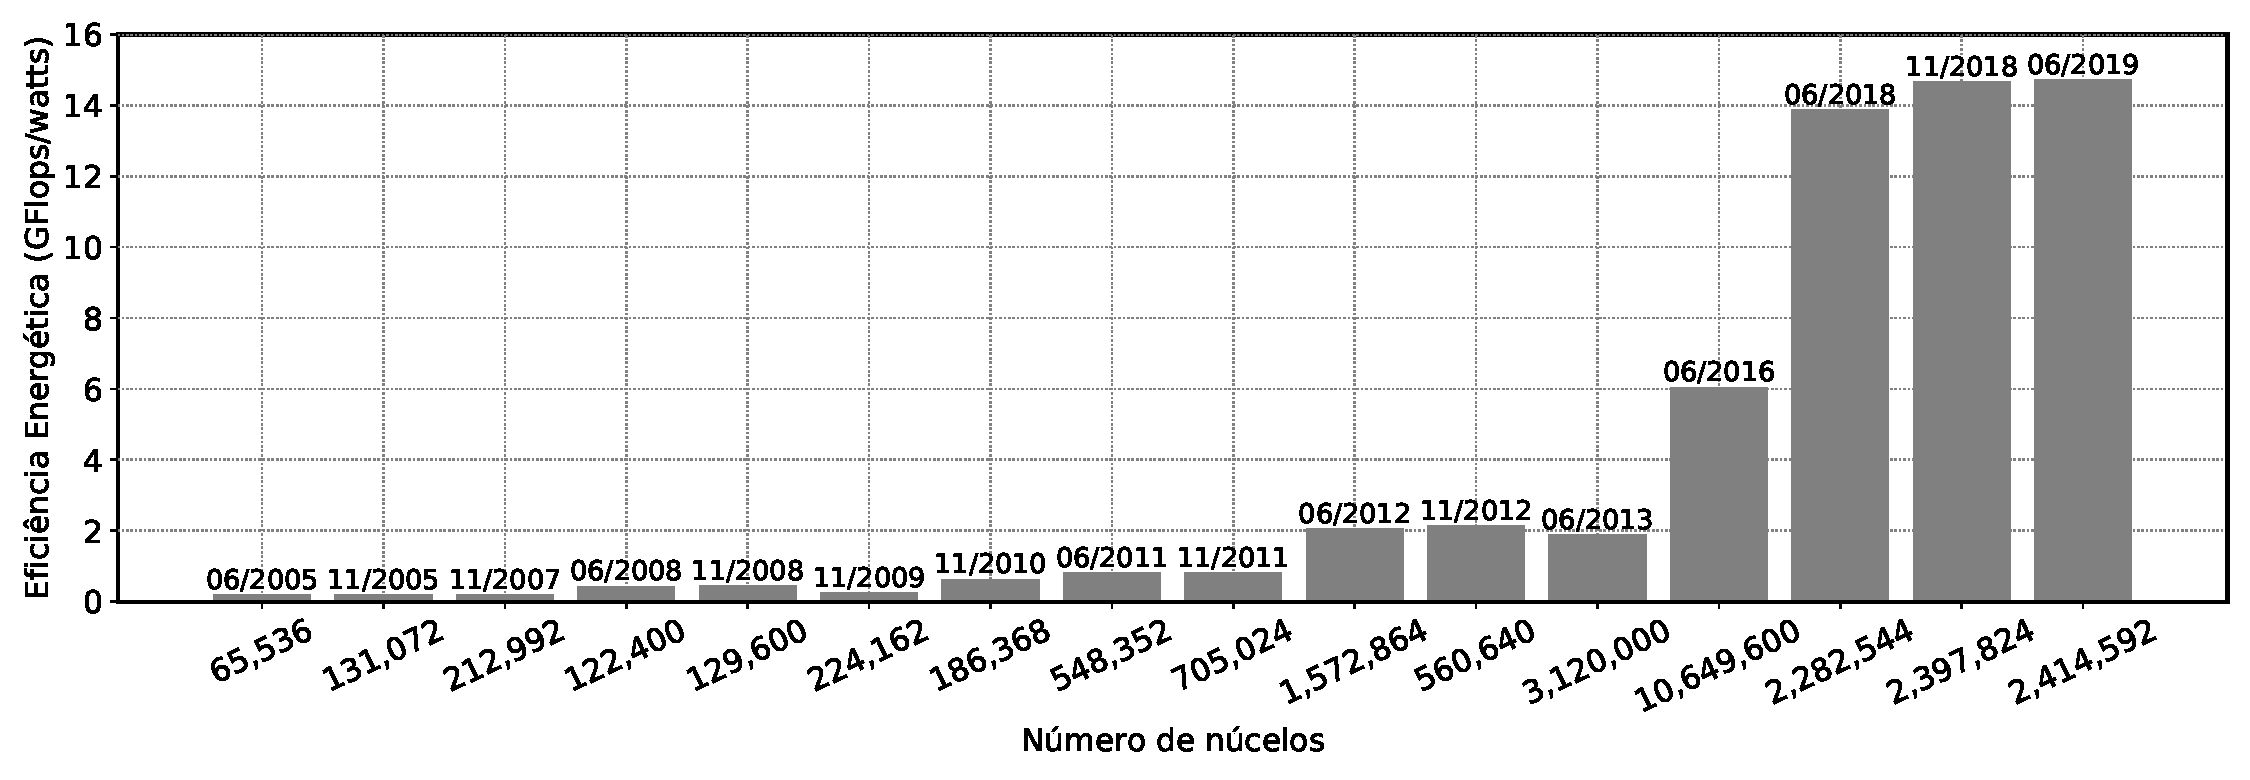
\includegraphics[width=1\linewidth, keepaspectratio]{Figure_Efficiency_X_Cores_Top500.pdf}
  \fonte{Gráfico desenvolvido pelo autor.}
\end{figure}

\begin{figure}[tb]
  \centering
  \caption{Evolução da eficiência energética do supercomputador número 1 do mundo segundo o \ranking TOP500.}
  \label{fig:eficienciaxyearstop500}
  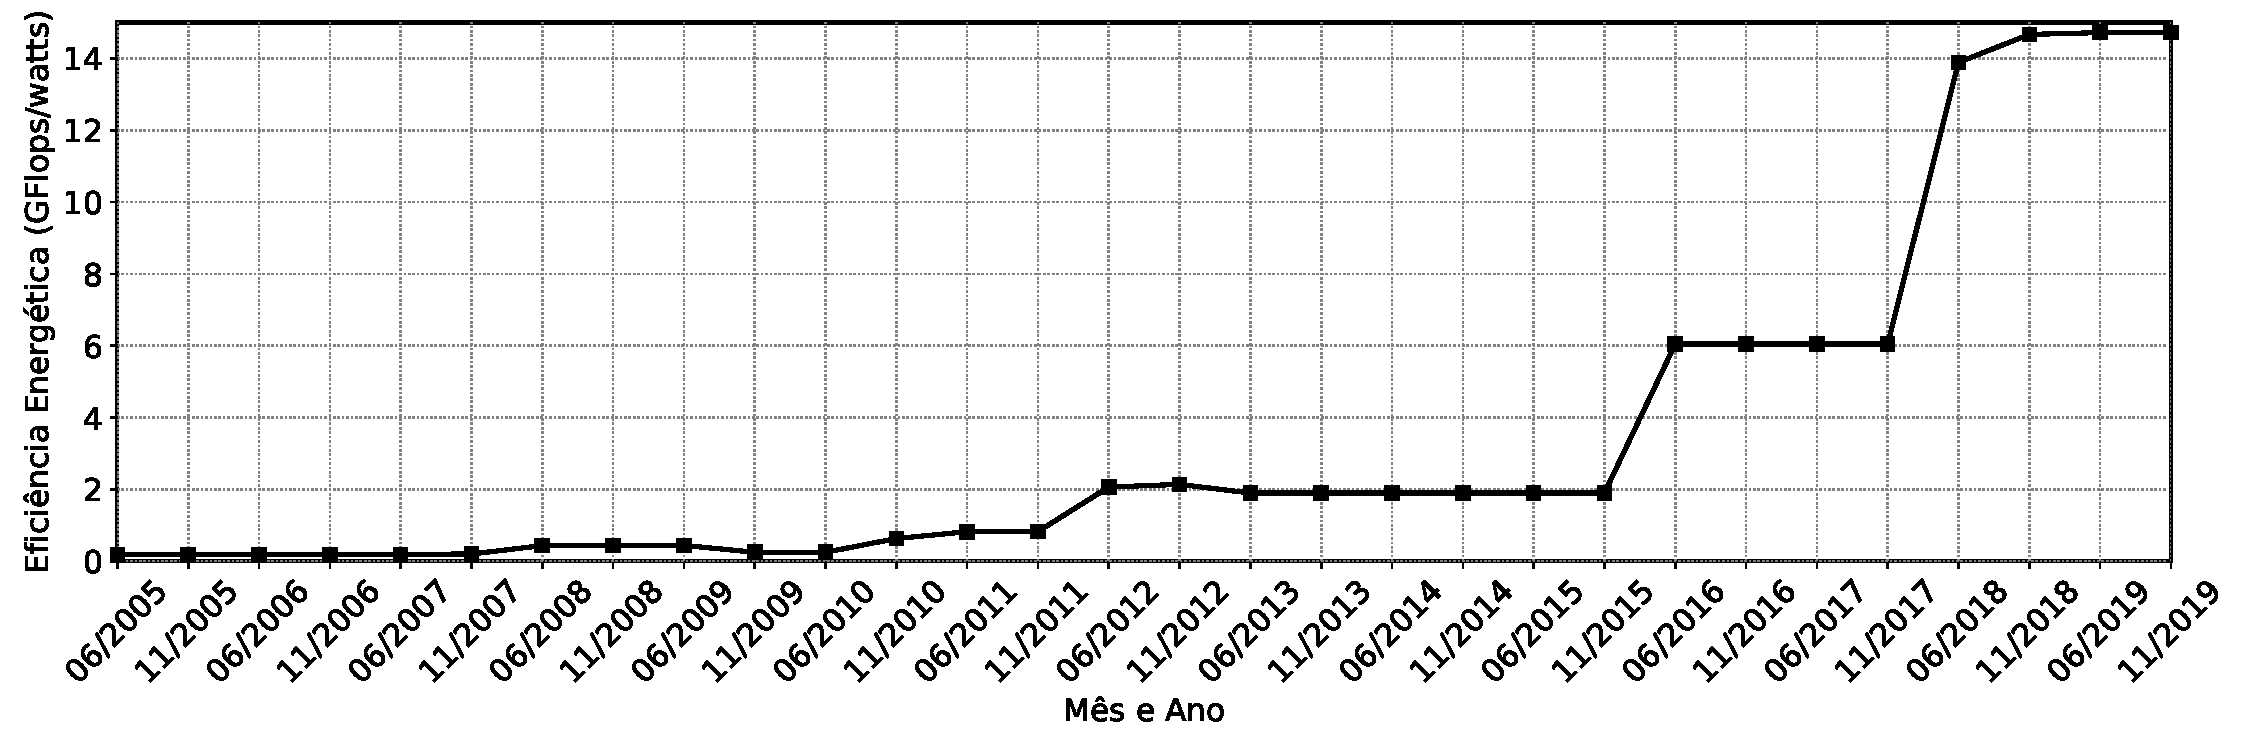
\includegraphics[width=1\linewidth, keepaspectratio]{Figure_Efficiency_X_Years_Top500.pdf}
  \fonte{Gráfico desenvolvido pelo autor.}
\end{figure}

Buscando novos tipos de arquiteturas paralelas que apresentem as características faltantes no problema de balanceamento apresentado acima, pesquisadores da área de \HPC realizaram diversos estudos voltados para essa questão, aplicando conceitos de \greencomputing \cite{greencomputingacm} no decorrer do desenvolvimento de suas soluções. Dentre estas soluções, temos o surgimento da classe de processadores \manycore de baixa potência, como o MPPA-256 \cite{mppa2562013}, objeto de estudo deste trabalho, o Adapteva Epiphany \cite{olofsson2014}, e o SW26010, utilizado no atual terceiro supercomputador mais poderoso do mundo, o \textit{Sunway TaihuLight} \cite{fu2016sunway}. Vale citar que o SW26010 desbancou em 2016 o supercomputador que assumia, desde 2013, a primeira posição do \ranking TOP500, obtendo duas vezes mais desempenho que esse e reduzindo em três vezes o consumo energético, explicando também o ganho elevado em eficiência em ambas as Figuras \ref{fig:eficienciaxcorestop500} e \ref{fig:eficienciaxyearstop500} no mês de junho de 2016.

Para avaliar o desempenho e consumo energético do MPPA-256, \textit{Souza} \etal propuseram o desenvolvimento do \bench \capb, o qual, em sua primeira versão, utilizava uma \API de comunicação síncrona entre processos denominada \IPC \cite{mppa2562013}. Essa \API possui algumas deficiências, como o baixo nível de abstração, requerendo conhecimento prévio da arquitetura alvo para implementações paralelas eficientes, e a realização de sincronizações implícitas muitas vezes não necessárias nas operações de envio e recebimento de dados, o que leva a queda de desempenho da aplicação. Ao realizar a otimização do \bench, \textit{David} \etal o portaram com a \ASYNC, uma \API com maior nível de abstração e com conceitos de assincronismo, aumentando o potencial de desempenho da aplicação. Além disso, alterações na implementação de todas as aplicações foram realizadas de modo a otimizá-las ainda mais.

Portanto, para realizar uma comparação justa entre as \APIs citadas acima, faz-se necessário atualizar a lógica de implementação das aplicações da versão antiga do \bench, para que essas se equivalham às novas implementações, criando assim um ambiente propício para comparar aspectos puramente das tecnologias de comunicação citadas, utilizando as duas versões do \bench para isso. A comparação entre ambas as implementações será responsável por determinar qual \API se comporta de maneira mais robusta no MPPA-256 em certos contextos, onde os dados acerca do tempo de execução, quantidade de dados enviados e recebidos e gasto energético de cada aplicação serão as métricas para essa determinação. Assim, teremos dados de execução das duas \APIs numa mesma versão de placa do MPPA-256, resultando numa base de dados concreta para a tomada de decisão sobre qual das duas \APIs escolher na hora de implementar uma nova aplicação.

\section{Objetivos}
\label{sec:objetivos}

Com base no que foi exposto, são apresentados abaixo o objetivo geral e os objetivos específicos deste trabalho.

\subsection{Objetivo Geral}
\label{sec:objetivogeral}

O objetivo deste trabalho é obter dados concretos acerca da execução de aplicações de diversos domínios de problemas no MPPA-256, utilizando as duas \APIs já citadas e o \capb, podendo assim comparar as execuções de cada aplicação em cada cenário específico possível dentro do processador, obtendo identificadores precisos que, em momentos futuros, possam apontar qual das duas \APIs utilizar, dependendo do domínio de problema de uma certa aplicação.

\subsection{Objetivos Específicos}
\label{sec:objetivosespecifico}

\begin{itemize}
\item Investigar a viabilidade do uso do MPPA-256 para a área de \HPC.
\item Estudar aspectos das \APIs de comunicação existentes no MPPA-256, mais especificamente, a \ASYNC e a \IPC.
\item Avaliar os custos e benefícios do MPPA-256 em relação ao desempenho e gasto energético, assim como sua utilidade para a Computação Sustentável (\greencomputing)
\item Comparar as \APIs \ASYNC e \IPC a fim de prover métricas precisas para a escolha de uma das duas numa futura implementação.
\end{itemize}

\section{Contribuições do trabalho}

Este trabalho é continuação de um projeto de iniciação científica desenvolvido por \textit{David} \etal, o qual resultou em um resumo expandido publicado na Escola Regional de Alto Desempenho da Região Sul no ano de 2019:

\begin{itemize}
  \item ORDINE, D. G. V.; PODESTA JUNIOR, E. ; PENNA, P. H. ; CASTRO, M. \textbf{Otimização de Aplicações do CAP Bench para o Processador MPPA-256.} In: Escola Regional de Alto Desempenho da Região Sul (ERAD/RS), 2019, Três de Maio. Anais da Escola Regional de Alto Desempenho da Região Sul (ERAD/RS). Porto Alegre: Sociedade Brasileira de Computação (SBC), 2019.
\end{itemize}

\section{Organização do trabalho}

Este trabalho está dividido da seguinte forma. O Capítulo \ref{ch:fundamentacaoteorica} mostra os conceitos teóricos que foram utilizados para a produção dessa dissertação. O Capítulo \ref{ch:trabcorrelatos} apresenta alguns trabalhos relacionados a este. O Capítulo \ref{ch:desenvolvimento} contém toda a proposta deste projeto, detalhando tudo que foi feito, assim como explicando as métricas que serão expostas nos resultados. O Capítulo \ref{ch:resultados} apresenta os resultados preliminares já obtidos. Para finalizar, o Capítulo \ref{ch:conclusao} conclui este trabalho.

\chapter{Fundamentação Teórica}
\label{ch:fundamentacaoteorica}

Neste capítulo são apresentados conceitos relacionados a Computação Paralela, por exemplo, padrões arquiteturais, na Seção \ref{sec:arquiteturasparalelas}, e tecnologias de programação, na Seção \ref{sec:bibliotecasdevparalelo}. Também são mostrados algumas características do MPPA-256 na Seção \ref{sec:mppa256}.

\section{Arquiteturas Paralelas}
\label{sec:arquiteturasparalelas}

Existem três tipos de sistemas com múltiplos processadores, segundo \textit{Tanenbaum} \etal : os multiprocessadores, os multicomputadores e os sistemas distribuídos \cite{TanenbaumMordenOS}. São detalhados nesta seção conceitos acerca das arquiteturas multiprocessadores e multicomputadores.

\subsection{Multiprocessadores}
\label{sec:multiprocessadores}

A principal característica de uma arquitetura multiprocessador é o acesso compartilhado ao barramento de memória do sistema, a \RAM, por diversas \CPUs. Programas executando em qualquer um dessas \CPUs possuem espaços de endereçamento físicos únicos na \RAM e as \threads de um desses programas fazem uso de um mesmo espaço de memória, através de operações de escrita e leitura, para se comunicarem. Um fato peculiar dessa arquitetura é a possibilidade de ocorrer problemas de concorrência quando duas ou mais \threads de um mesmo programa executam em diferentes \CPUs, onde, na visão de uma \CPU, ela escreve um valor em uma posição de memória e lê outro valor daquela mesma posição, pois uma \thread executando em outra \CPU alterou o valor daquela posição. 

Multiprocessadores são também classificados em dois tipos, de acordo com a velocidade de acesso a uma posição de memória. Quando uma certa palavra na memória pode ser lida na mesma velocidade que qualquer outra, são chamados de multiprocessadores com acesso uniforme a memória - \UMA. Já quando a velocidade de leitura em diferentes posições de memória muda, são chamados de multiprocessadores com acesso não uniforme a memória - \NUMA. 

A arquitetura mais simples de um multiprocessador \UMA, exemplificada na Figura \ref{fig:umasimples}, envolve um único barramento conectando duas ou mais \CPUs a um módulo de memória, permitindo que todas as \CPUs realizem operações de leitura e escrita neste módulo. Quando uma \CPU necessita ler alguma palavra da memória, primeiramente ela verifica se o barramento está ocupado. Caso não, informa à memória, através do barramento, qual endereço deseja obter o valor, aguardando o recebimento deste pelo mesmo barramento. Caso esteja, a \CPU aguarda a liberação do barramento. Para uma pequena quantidade de \CPUs, o tempo de espera médio para o acesso ao barramento tende a ser pequeno e tolerável. Porém, quando elevam-se em algumas dezenas o número de \CPUs observa-se o principal problema deste exemplo de arquitetura \UMA: a ociosidade, por muito tempo, de grande parte das \CPUs, enquanto aguardam pelo acesso ao barramento.



\begin{figure}[tb]
  \centering
  \caption{Diferentes esquemas possiveis de um multiprocessador UMA baseado em barramento.}
  \subcaptionminipage[fig:umasimples]%
    {.4\linewidth}%
    {Sem \textit{cache}}%
    {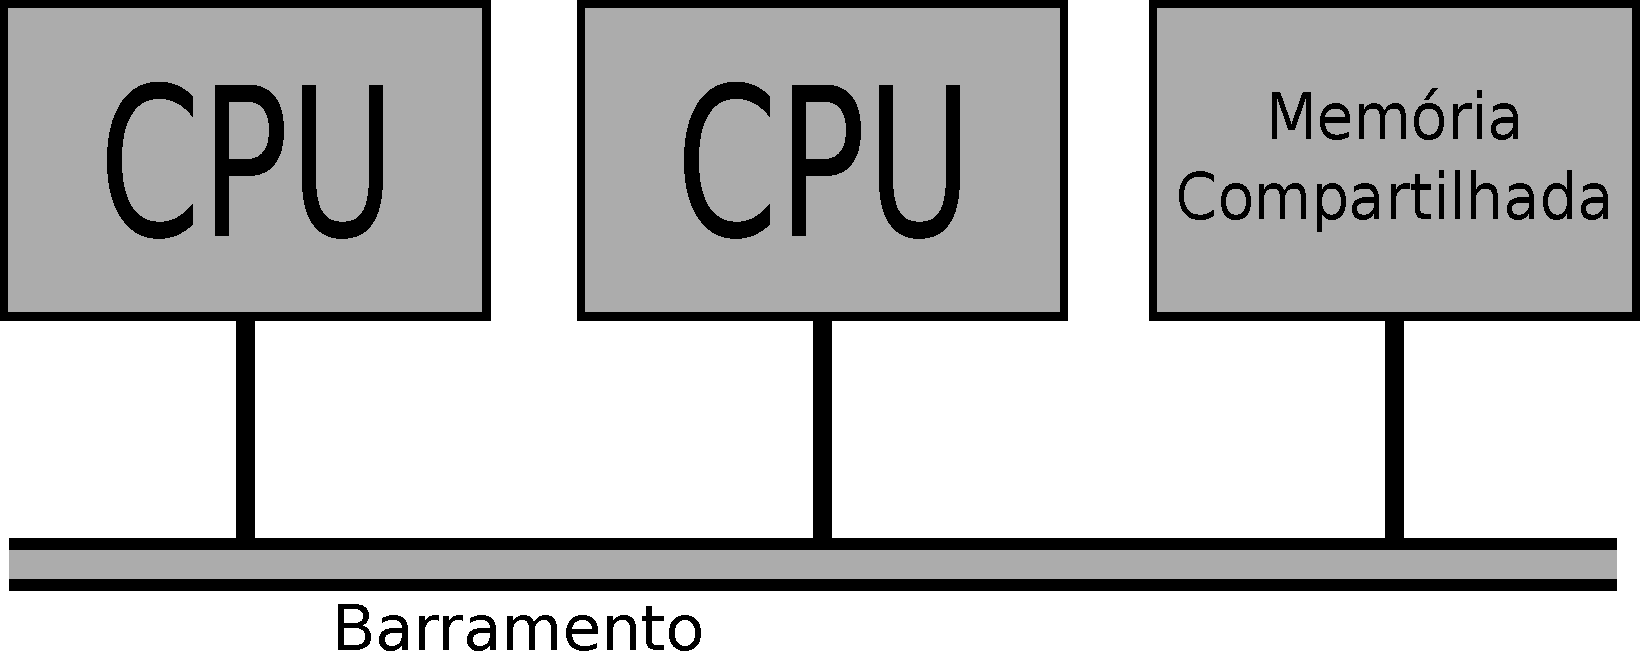
\includegraphics[width=.9\linewidth]{umasimples.pdf}}%
  \hfill% 
  \subcaptionminipage[fig:umacomcache]%
    {.4\linewidth}%
    {Com \textit{cache}}%
    {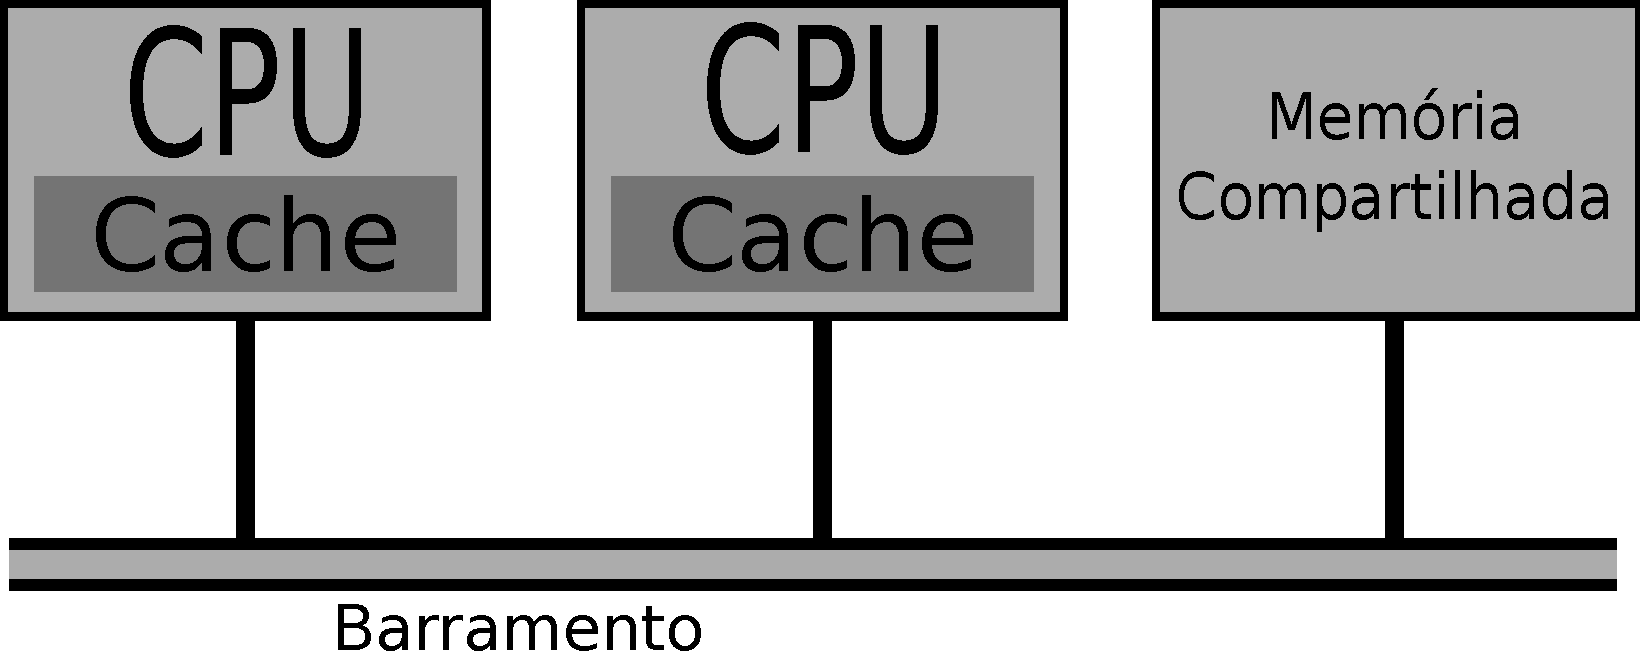
\includegraphics[width=.9\linewidth]{umacomcache.pdf}}%
  \hfill% 
  \subcaptionminipage[fig:umacomcacheememprivada]%
    {.4\linewidth}%
    {Com \textit{cache} e memórias privadas}%
    {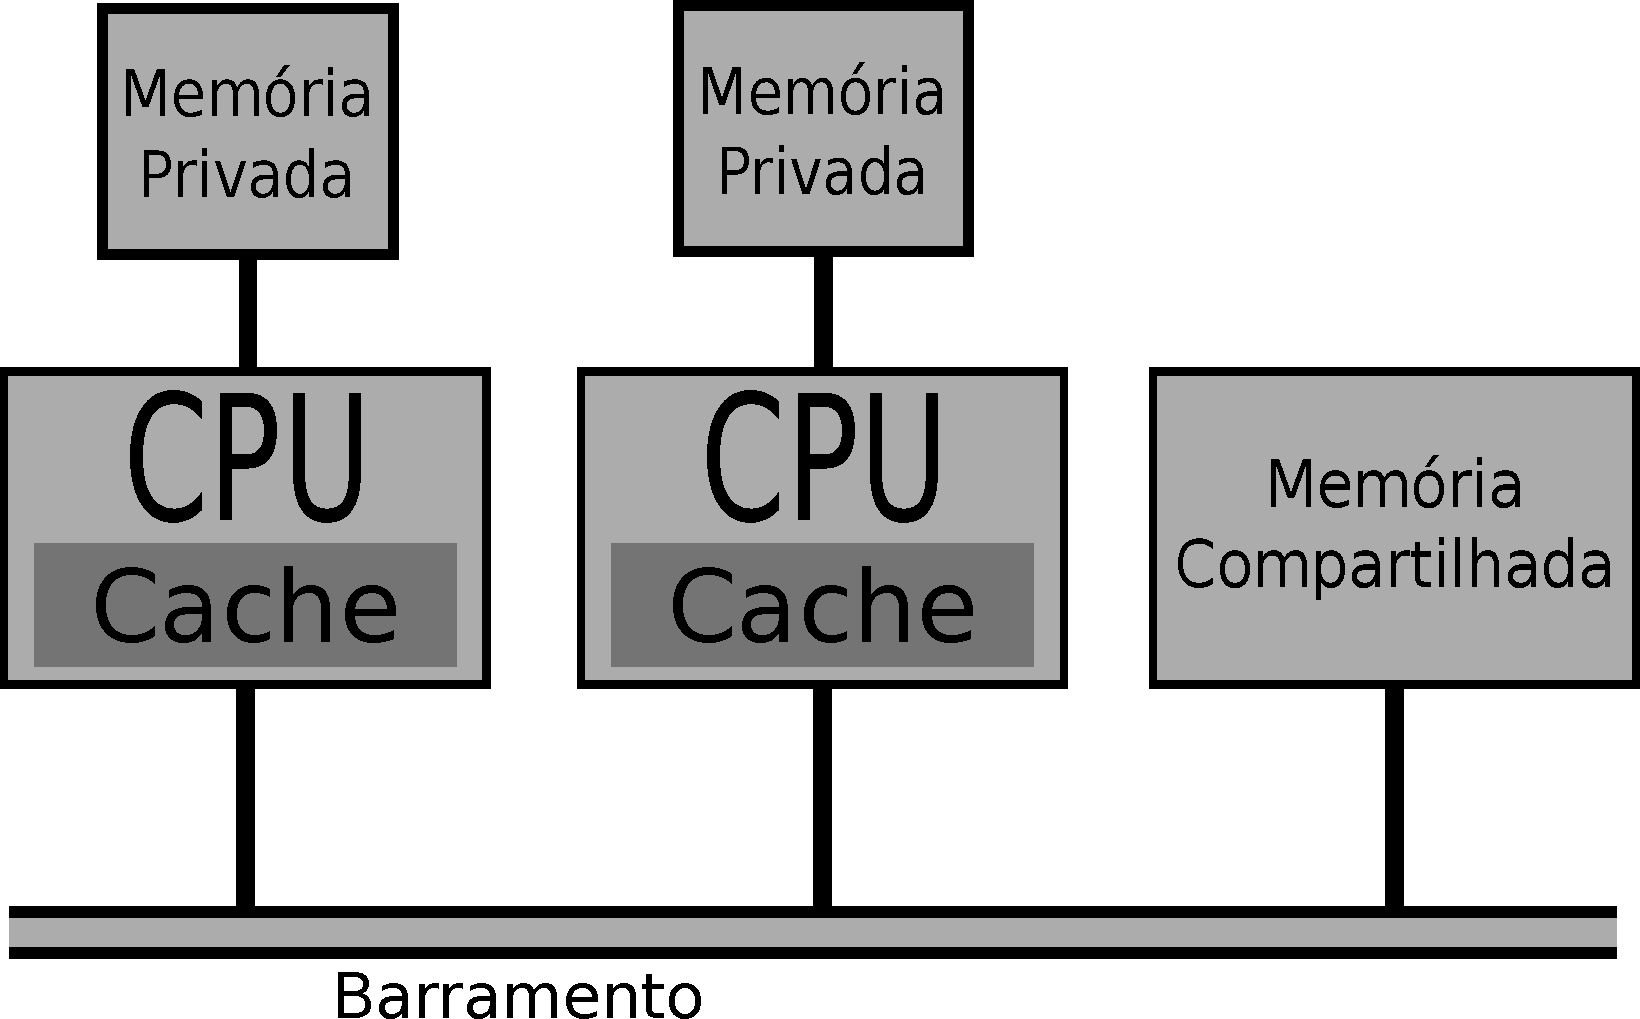
\includegraphics[width=.9\linewidth]{umacomcacheememprivada.pdf}}%
  \hfill% 
  \fonte{Imagens desenvolvidas pelo autor, adaptadas de \textit{Tanenbaum} \etal \cite{TanenbaumMordenOS}.}
\end{figure}

Adicionar \caches às \CPUs, como na Figura \ref{fig:umacomcache}, é uma solução para reduzir o gargalo imposto sobre o barramento, já que agora valores podem ser lidos diretamente da \cache local, a qual está muito mais próxima da \CPU e possui tempo de acesso muito menor. Outra possibilidade é adicionar, além das \caches, memórias privadas locais,  como na Figura \ref{fig:umacomcacheememprivada}. Compiladores podem colocar nessas memórias todos os dados que são somente de leitura, por exemplo, constantes, o código do programa, strings e pilhas, utilizando assim esta segunda configuração de forma otimizada. Ambas configurações removem grande parte do tráfego no barramento, tornando seu uso exclusivamente para as variáveis compartilhadas entre \threads.

A adição de \caches impõe uso de protocolos de coerência para que não haja inconsistência entre os valores de um mesmo endereço de memória nas diferentes \caches. Primeiramente, para otimizar as operações de leitura, quando uma palavra é referenciada, todo o bloco que contém essa palavra, geralmente de 32 ou 64 \bytes, é colocado na \cache. Já para garantir a coerência, cada bloco é marcado como sendo somente de leitura, podendo assim estar presente em outras \caches, ou de leitura e escrita, não devendo estar presente em nenhuma outra \cache neste caso. Quando uma \CPU tenta alterar um valor que está presente em outras \caches além de sua própria, o \hardware do barramento informa essa operação às outras \caches, as quais tratam esse contexto de duas formas. Caso o valor da \cache seja o mesmo em memória, podem simplesmente descartá-lo, buscando o novo valor na memória se necessário. Caso outra \cache tenha um valor diferente daquele em memória, é necessário ou salvá-lo na memória ou transferi-lo diretamente para a \cache que solicitou a operação de escrita.

Quando necessita-se de um número de processadores na ordem das centenas, a arquitetura \UMA acaba sendo inviável. Assim, introduz-se a arquitetura \NUMA, trazendo com ela a ideia de diferentes tempos de acesso para diferentes posições de memória. Multiprocessadores \NUMA provém essa escalabilidade implementando um espaço de endereçamento único para todas as \CPUs através de uma rede de interconexão, como na Figura \ref{fig:multiprocessadornuma}, o que causa a diferença nos tempos de acesso, os quais serão totalmente dependentes do local da memória que se deseja acessar um valor relativo ao local da \CPU que requisitou este acesso. Logo, outra propriedade desta arquitetura é o acesso mais rápido à memória local de um ou um conjunto de \CPUs, em comparação com o acesso à memória remota. Vale salientar que programas desenvolvidos para multiprocessadores \UMA conseguem ser executados em arquiteturas \NUMA, devido a ambas possuírem um espaço de endereçamento único. Porém, estes programas irão obter performance inferior, já que não foram otimizados para considerar as diferenças de tempo entre acesso à memória local e remota.

\begin{figure}[tb]
  \centering
  \caption{Esquema genérico de um multiprocessador NUMA.}
  \label{fig:multiprocessadornuma}
  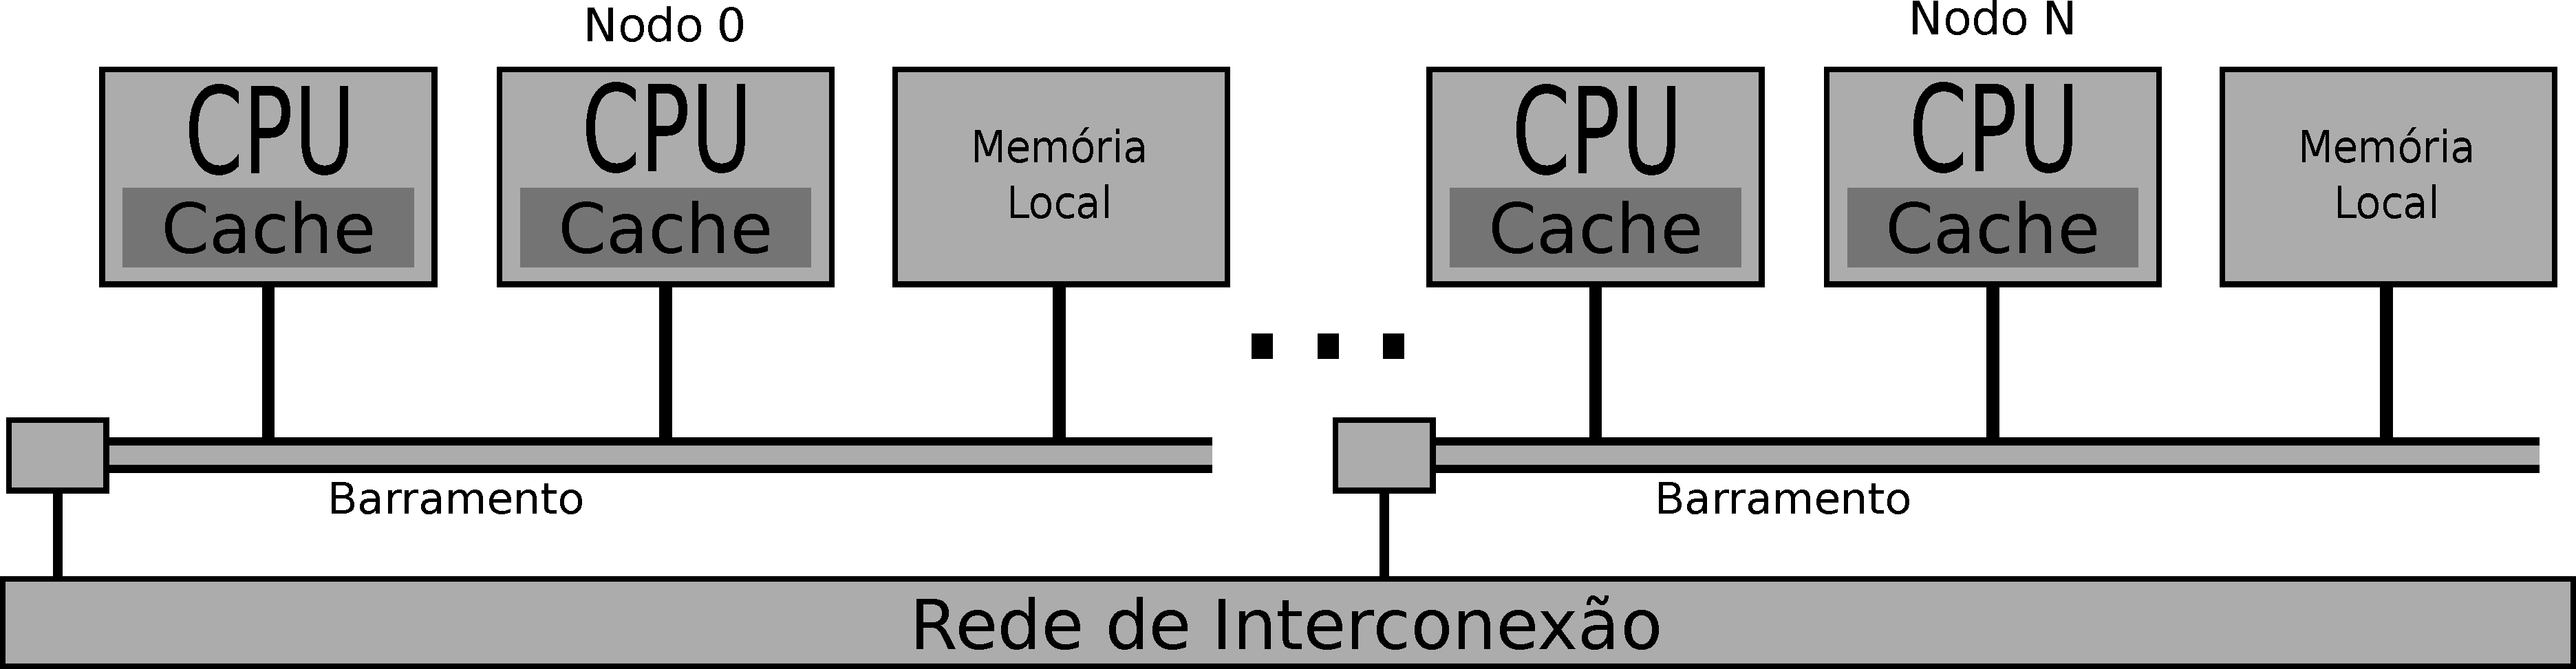
\includegraphics[width=.9\linewidth, keepaspectratio]{numa.pdf}
  \fonte{Imagem desenvolvida pelo autor, adaptada de \textit{Tanenbaum} \etal \cite{TanenbaumMordenOS}.}
\end{figure}

A medida que o tamanho de um \transistor diminui, o número de \transistors em um \chip tende a aumentar. Diversas soluções exploram o que fazer com este número crescente de \transistors, por exemplo, adicionar \caches poderosas de muitos \textit{mega}\bytes ou colocar duas ou mais \CPUs, também chamadas de núcleos (em inglês \textit{cores}), neste mesmo \chip. Em certo ponto, o aumento no tamanho da \cache traz pouquíssimo ganho em porcentagem de \textit{hit} (quantidade de vezes que é possível buscar um dado diretamente na \cache), mostrando assim que o investimento no paralelismo trazido pelos múltiplos núcleos como recurso para ganho em desempenho é uma opção a se considerar. Assim, \chips \multicore são uma mescla de múltiplas \CPUs com múltiplos níveis de \cache inseridos em um espaço muito menor que um multiprocessador, sendo por isso também chamados de \CMPs.

Apesar de serem parecidos, existem algumas diferenças entre os \CMPs e os multiprocessadores. Primeiramente, em muitos \CMPs ocorre o compartilhamento da \cache nível 2 ou 3 entre suas \CPUs, o que não acontece nos multiprocessadores, que possuem \caches totalmente privadas em todos os níveis. Além disso, a probabilidade de que falhas em componentes compartilhados levem a impossibilidades em múltiplas \CPUs ao mesmo tempo é muito maior nos \CMPs, devido a proximidade de conexão das \CPUs. Por fim, existem \chips \multicore em que todos os núcleos são feitos para atender a uma ampla gama de contextos, enquanto que em outros, além das \CPUs principais, existem também núcleos específicos para alguns problemas, como decodificação de áudio e vídeo ou interfaces de rede. 

Apesar de não haver uma barreira de distinção entre um \chip \manycore ou \multicore, pode-se chama-lo de \manycore quando a perda de um núcleo tem um pequeno impacto na performance total do \chip. Um problema com arquiteturas \manycore é a escalabilidade entre manter as \caches de todas as \CPUs coerentes e ainda assim elevar o desempenho ao elevar o número de núcleos. Cientistas da área de \HPC temem que essas duas variaveis não escalem proporcionalmente, tornando o custo de gerenciar essas \caches tão alto que a adição de um novo núcleo de pouco ajudara no aumento em performance. Este problema é também conhecido como a barreira de coerencia  (\textit{coherency wall}) \cite{TanenbaumMordenOS}.

Para o futuro dos \manycore, espera-se processadores que invistam mais  na comunicação entre \CPUs através da troca de mensagens extremamente rápidas via \hardware e através de uma memória compartilhada, deixando de lado parte da coerência de \cache. Uma \GPU é um dos exemplos mais comuns de um processador \manycore, possuindo milhares de pequenos núcleos especializados na rápida execução de cálculos e sem uma lógica complexa de \cache, ou seja, priorizam o processamento. Desta maneira, \GPUs são excepcionais para a execução paralela de pequenas tarefas, como a renderização de \textit{frames} para jogos. Programar para uma \GPU é uma tarefa difícil e muitas vezes algumas linguagens de programação especiais são utilizadas, como a OpenGL ou a CUDA, da NVIDIA. Essa dificuldade se dá, principalmente, pelo fato dos núcleos de uma \GPU executarem exatamente a mesma instrução em diferentes fatias de um dado, ou seja, pelo fato da \GPU ser uma máquina \SIMD.

\subsection{Multicomputadores}
\label{sec:multicomputadores}

Multicomputadores surgiram na dificuldade de aumentar o poder de processamento de um multiprocessador quando se atinge grandes escalas em relação ao número de núcleos. Ao contrário dos multiprocessadores, multicomputadores não compartilham memória, sendo relativamente fáceis de se construir, tendo como componente principal um computador com uma placa de rede de alta performance, sem mouse, teclado e monitor. Neste sistema, também chamado de \textit{Cluster Computers} ou {Cluster Of Workstations} (COWs), é necessário um \textit{design} inteligente da rede que irá conectar os computadores para que se possa obter um alto desempenho.

Um nó de um multicomputador consiste então em um computador, com uma \CPU, memória, placa de rede e um HD. Diversas são as topologias possíveis para a rede que conecta os nós, como mostrado na Figura \ref{fig:topologiamulticomputadores}. Sistemas pequenos utilizam-se de apenas um \textit{switch} para conectar os nós entre si, os quais são então organizados em forma de estrela, como na Figura \ref{fig:topologiamulticomputadores}(a). Também é possível organizar os nós em forma de anel, onde cada nó se conecta aos nós da sua esquerda e direita, como na Figura \ref{fig:topologiamulticomputadores}(b), eliminando a necessidade de um \textit{switch}. Porém, o problema dessas arquiteturas é a escalabilidade, a qual dificulta o ganho em desempenho a medida que se aumenta o número de nós devido ao tempo de viagem dos dados entre nós.

\begin{figure}[tb]
  \centering
  \caption{Tipos de topologias de rede de multicomputadores.}
  \label{fig:topologiamulticomputadores}
  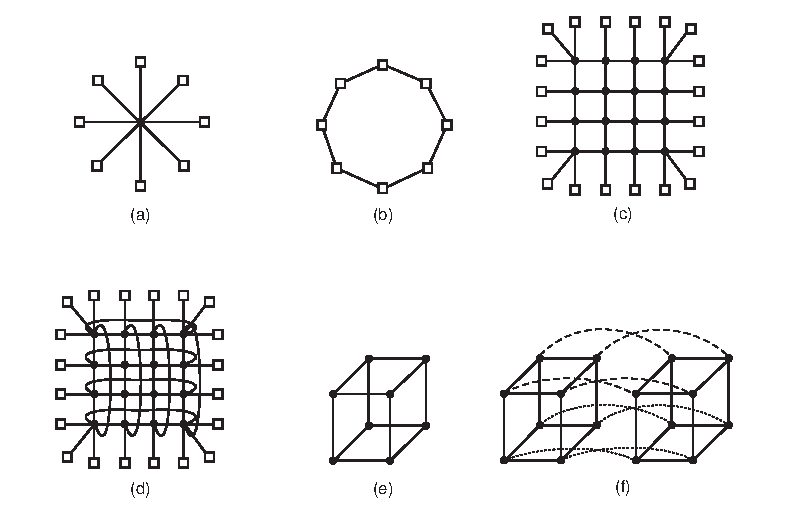
\includegraphics[width=.9\linewidth, keepaspectratio]{topologia.pdf}
  \fonte{\cite{TanenbaumMordenOS}.}
\end{figure}

Topologias mais complexas, como a malha (\textit{grid} ou \textit{mesh}), mostrada na Figura \ref{fig:topologiamulticomputadores}(c), ou a \textit{double torus}, mostrada na Figura \ref{fig:topologiamulticomputadores}(d), são mais escaláveis do que as apresentadas anteriormente. Nessas topologias, os nós são conectados em \textit{switches} e estes são conectados entre si, formando um \textit{layout} de malha no sistema. Dentre as duas citadas, a \textit{double torus} é mais escalável devido a conexão entre nós nas arestas da rede, trazendo assim conexões extras ao sistema, o que aumenta a tolerância a faltas e o desempenho, já que o caminho entre estes nós se torna menor. Este tipo de rede possui uma propriedade chamada de diâmetro, que é o caminho mais longo entre dois nós. Para topologias bidimensionais como a malha, o diâmetro aumenta proporcionalmente a raiz quadrada do número de nós. \textit{Layouts} \textit{n} dimensionais, como mostrado na Figura \ref{fig:topologiamulticomputadores}(e) (tridimensional) e na Figura \ref{fig:topologiamulticomputadores}(f) (quadrimensional), são ainda mais escaláveis, já que o diâmetro diminui à medida que se aumenta o número de dimensões da rede, tendo como única desvantagem o custo elevado, devido ao grande número de ligações presentes entre nós e \textit{switches}.

A comunicação entre processos rodando em diferentes \CPUs, num multicomputador, se dá através da troca de mensagens entre estes. Basicamente, o \SO presente no multicomputador é o responsável por realizar essa troca, através de funções acessíveis somente a ele. Porém, bibliotecas podem fornecer abstrações a essas funções, tornando a troca de mensagens também disponível para os processos usuário e as simplificando, visto que abstraem toda uma lista de invocações de funções em uma única função. Essa troca de mensagens pode ser reduzida a duas funções, chamadas de \textit{send} e \textit{receive}. A função \textit{send} é responsável por enviar uma mensagem de uma \CPU para outra, passando parâmetros como o destino da mensagem e o endereço onde aquela mensagem se encontra. Já a função \textit{receive} é responsável por receber a mensagem, tendo como parâmetros, por exemplo, o endereço de onde a mensagem será lida e o endereço onde será armazenada. Por fim, essas funções podem ser síncronas, bloqueando o processo que envia ou recebe a mensagem até que a operação seja concluída, ou assíncronas, não bloqueando o processo que realizou tal operação.

\section{MPPA-256}
\label{sec:mppa256}

\section{Desenvolvimento de Aplicações Paralelas}
\label{sec:bibliotecasdevparalelo}

\subsection{Bibliotecas multiplataforma}
\label{sec:bibliotecasmultiplataforma}

\subsection{Bibliotecas específicas para o MPPA-256}
\label{sec:bibliotecasespecificasmppa}

\chapter{Trabalhos Correlatos}
\label{ch:trabcorrelatos}


\section{Benchmarks Voltados para HPC}
\label{sec:benchprahpc}

\section{Benchmarks Específicos para Manycores}
\label{sec:benchpramanycores}

\chapter{Desenvolvimento}
\label{ch:desenvolvimento}

\chapter{Resultados}
\label{ch:resultados}

\chapter{Conclusão}
\label{ch:conclusao}

\index{bobagem} Primeiro parágrafo da seção com uma frase sem sentido que só serve para ocasionar uma quebra e de demonstrar a configuração de indentação da primeira linha. Essa frase está aqui pois parágrafos de uma linha são feios.

Resultado do uso de siglas:
\begin{itemize}
\item Sigla que nunca expande: \API;
\item Sigla normal, expande no primeiro uso: \DHT, mas não no segundo: \DHT;
\item Siglas com plurais automaticos: \APIs e \DHTs;
\item Plural não-trivial: \SQs;
\item Forçando uma expansão (e no plural) \Glsfirstplural{DHT};
\item Usando uma sigla cujo comando é diferente da sigla: \WTC.
\end{itemize}

Resultado do glossário:
\begin{itemize}
\item Dois termos, \polling e \proxy;
\item Plural: \proxys.
\end{itemize}

Resultado de \mla|index|: primeiro um link normal \indexterm{tomate}, depois um capitalizado \indexTerm{tomate}.

\begin{defn}
  Exemplo de definição
\end{defn}

\begin{theorem}
  Exemplo de teorema
\end{theorem}

\begin{theoremproof}
  Exemplo de prova \qed
\end{theoremproof}

(Sub)enumerações e citações (verificar se OK com o idioma):
\begin{enumerate}
\item \cite{turing1937}:
  \begin{enumerate}
  \item \citeonline{turing1937}:
    \begin{enumerate}
    \item \citeonline{dijkstra1968};
    \end{enumerate}
  \end{enumerate}
\item \cite{turing1937,dijkstra1968};
\item \citeonline{turing1937,dijkstra1968}.
\end{enumerate}


\begin{listing}[tb]
\caption{Meta informações do presente documento.}
\label{lst:meta}
\begin{minted}[highlightlines={1,4-5}]{latex}
\titulo{Template \LaTeX{} para testes e dissertações do LAPESD/UFSC}
\autor{Omar Ravenhurst}
\data{1 de agosto de 2019} % ou \today
\tese % ou \dissertacao
\titulode{Doutor em Ciência da Computação}
\orientador{Prof. Ben Trovato, Dr.}
\coorientador{Prof. Lars Thørväld, Dr.}

\membrobanca{Prof. Valerie Béranger, Dr.}{Universidade Federal de Santa Catarina}
\membrobanca{Prof. Mordecai Malignatus, Dr.}{Universidade Federal de Santa Catarina}
\membrobanca{Prof. Huifen Chan, Dr.}{Universidade Federal de Santa Catarina}
\coordenador{Prof. Charles Palmer, Dr.}
\end{minted}
\fonte{o autor.}
\end{listing}


Resultado de \mla|\autoref|s:
\begin{itemize}
\item \autoref{lst:meta};
\item \autoref{alg:algoritmo};
\item \autoref{fig:figura} tem subfiguras:
  \begin{itemize}
  \item \autoref{fig:svg}
  \item \autoref{fig:brasao}
  \end{itemize}
\item \autoref{tb:tabela};
\item \autoref{ch:exemplo};
\item \autoref{sec:frutas};
\item \autoref{sec:goiaba};
\item \autoref{sec:jabuticaba};
\item \autoref{sec:tomate}.
\end{itemize}


\begin{algorithm}
  \caption{Exemplo do ambiente \texttt{algorithimic}.}
  \label{alg:algoritmo}
  \begin{algorithmic}[1]
    \Procedure{Closure}{C, A}
      \State{$H \gets \emptyset$}\Comment{Direct cache}
      \For{$i \in [1, n]$}\Comment{Parallel, (dynamic,32) scheduling}
        \State{$H \gets H \cup \Call{DoImportantStuff}{i}$}
      \EndFor
    \EndProcedure
  \end{algorithmic}
  \fonte{o autor.}
\end{algorithm}

\begin{figure}[tb]
  \centering
  \caption{Exemplo de figura com duas subfiguras.}   
  \label{fig:figura}
  
  % Subfiguras são feitas usando as funcionalidades do memoir. Não
  % inclua outros pacotes, pois eles podem fazer o memoir dar ragequit
  % 
  % Há duas maneiras, a maneira limpinha (só no lapesd-thesis.cls) e a
  % maneira do memoir (aviso: \subtop não funciona direito).
  \subcaptionminipage[fig:svg]%
    {.49\linewidth}%
    {O Makefile compila SVGs em PDFs usando o inkscape}%
    {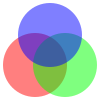
\includegraphics[width=.2\linewidth]{alphachannel.pdf}}%
  \hfill% 
  % o comando acima expande para o equivalente disso:
  \begin{minipage}[t]{.49\linewidth}%
    \centering
    \subcaption{Brasão da UFSC.\label{fig:brasao}}
    \includegraphics[width=.2\linewidth]{\jobname-logo.pdf}
  \end{minipage}

  \fonte{o autor.}
\end{figure}

\begin{table}[tb]
  \centering
  \caption{Exemplo de tabela e símbolos}
  \label{tb:tabela}
  \begin{tabular}{lccp{5cm}}
    \toprule
    Esquerda & Coluna 1    & \rotatebox{90}{90 graus}  & Parágrafo com \mla|p{5cm}|   \\
    \midrule
    $r_1$    & \cmk        &  \xmk                     & \circledi    \\
    $r_2$    &     \multicolumn{2}{c}{merged cell}     & \circledii   \\
    $r_3$    & \circlediii & \circlediv                & \circledv    \\
    $r_4$    & \circledvi  & \circledvii               & \circledviii \\
    $r_5$    & \circledix  &  x                        & y           \\
    \bottomrule 
  \end{tabular}
  \fonte{o autor.}
\end{table}

\begin{figure}[tb]
  \centering
  \caption{Segunda Figura.}
  \label{fig:segunda-fig}
  \includegraphics[width=.2\linewidth]{\jobname-logo.pdf}
  \fonte{o autor.}
\end{figure}

\xindex{tomate} \lipsum[4]


%%% Local Variables:
%%% mode: latex
%%% TeX-master: "main"
%%% End:

\postextual
% Assume-se que \postextual já foi feito

\apendices

\chapter{Exemplo de Apêndice}
\label{ch:apendice}

\lipsum[1]

\imprimirglossario

\imprimirindice


%%% Local Variables:
%%% mode: latex
%%% TeX-master: "main"
%%% End:


\bibliography{main}

\end{document}
